\section{Background and Related Work}
In this section, we present the necessary background knowledge about matrix factorization and unstructured pruning (\figref{fig:intro}).

\begin{figure}[t!]
	\centering
	\scalebox{0.154}{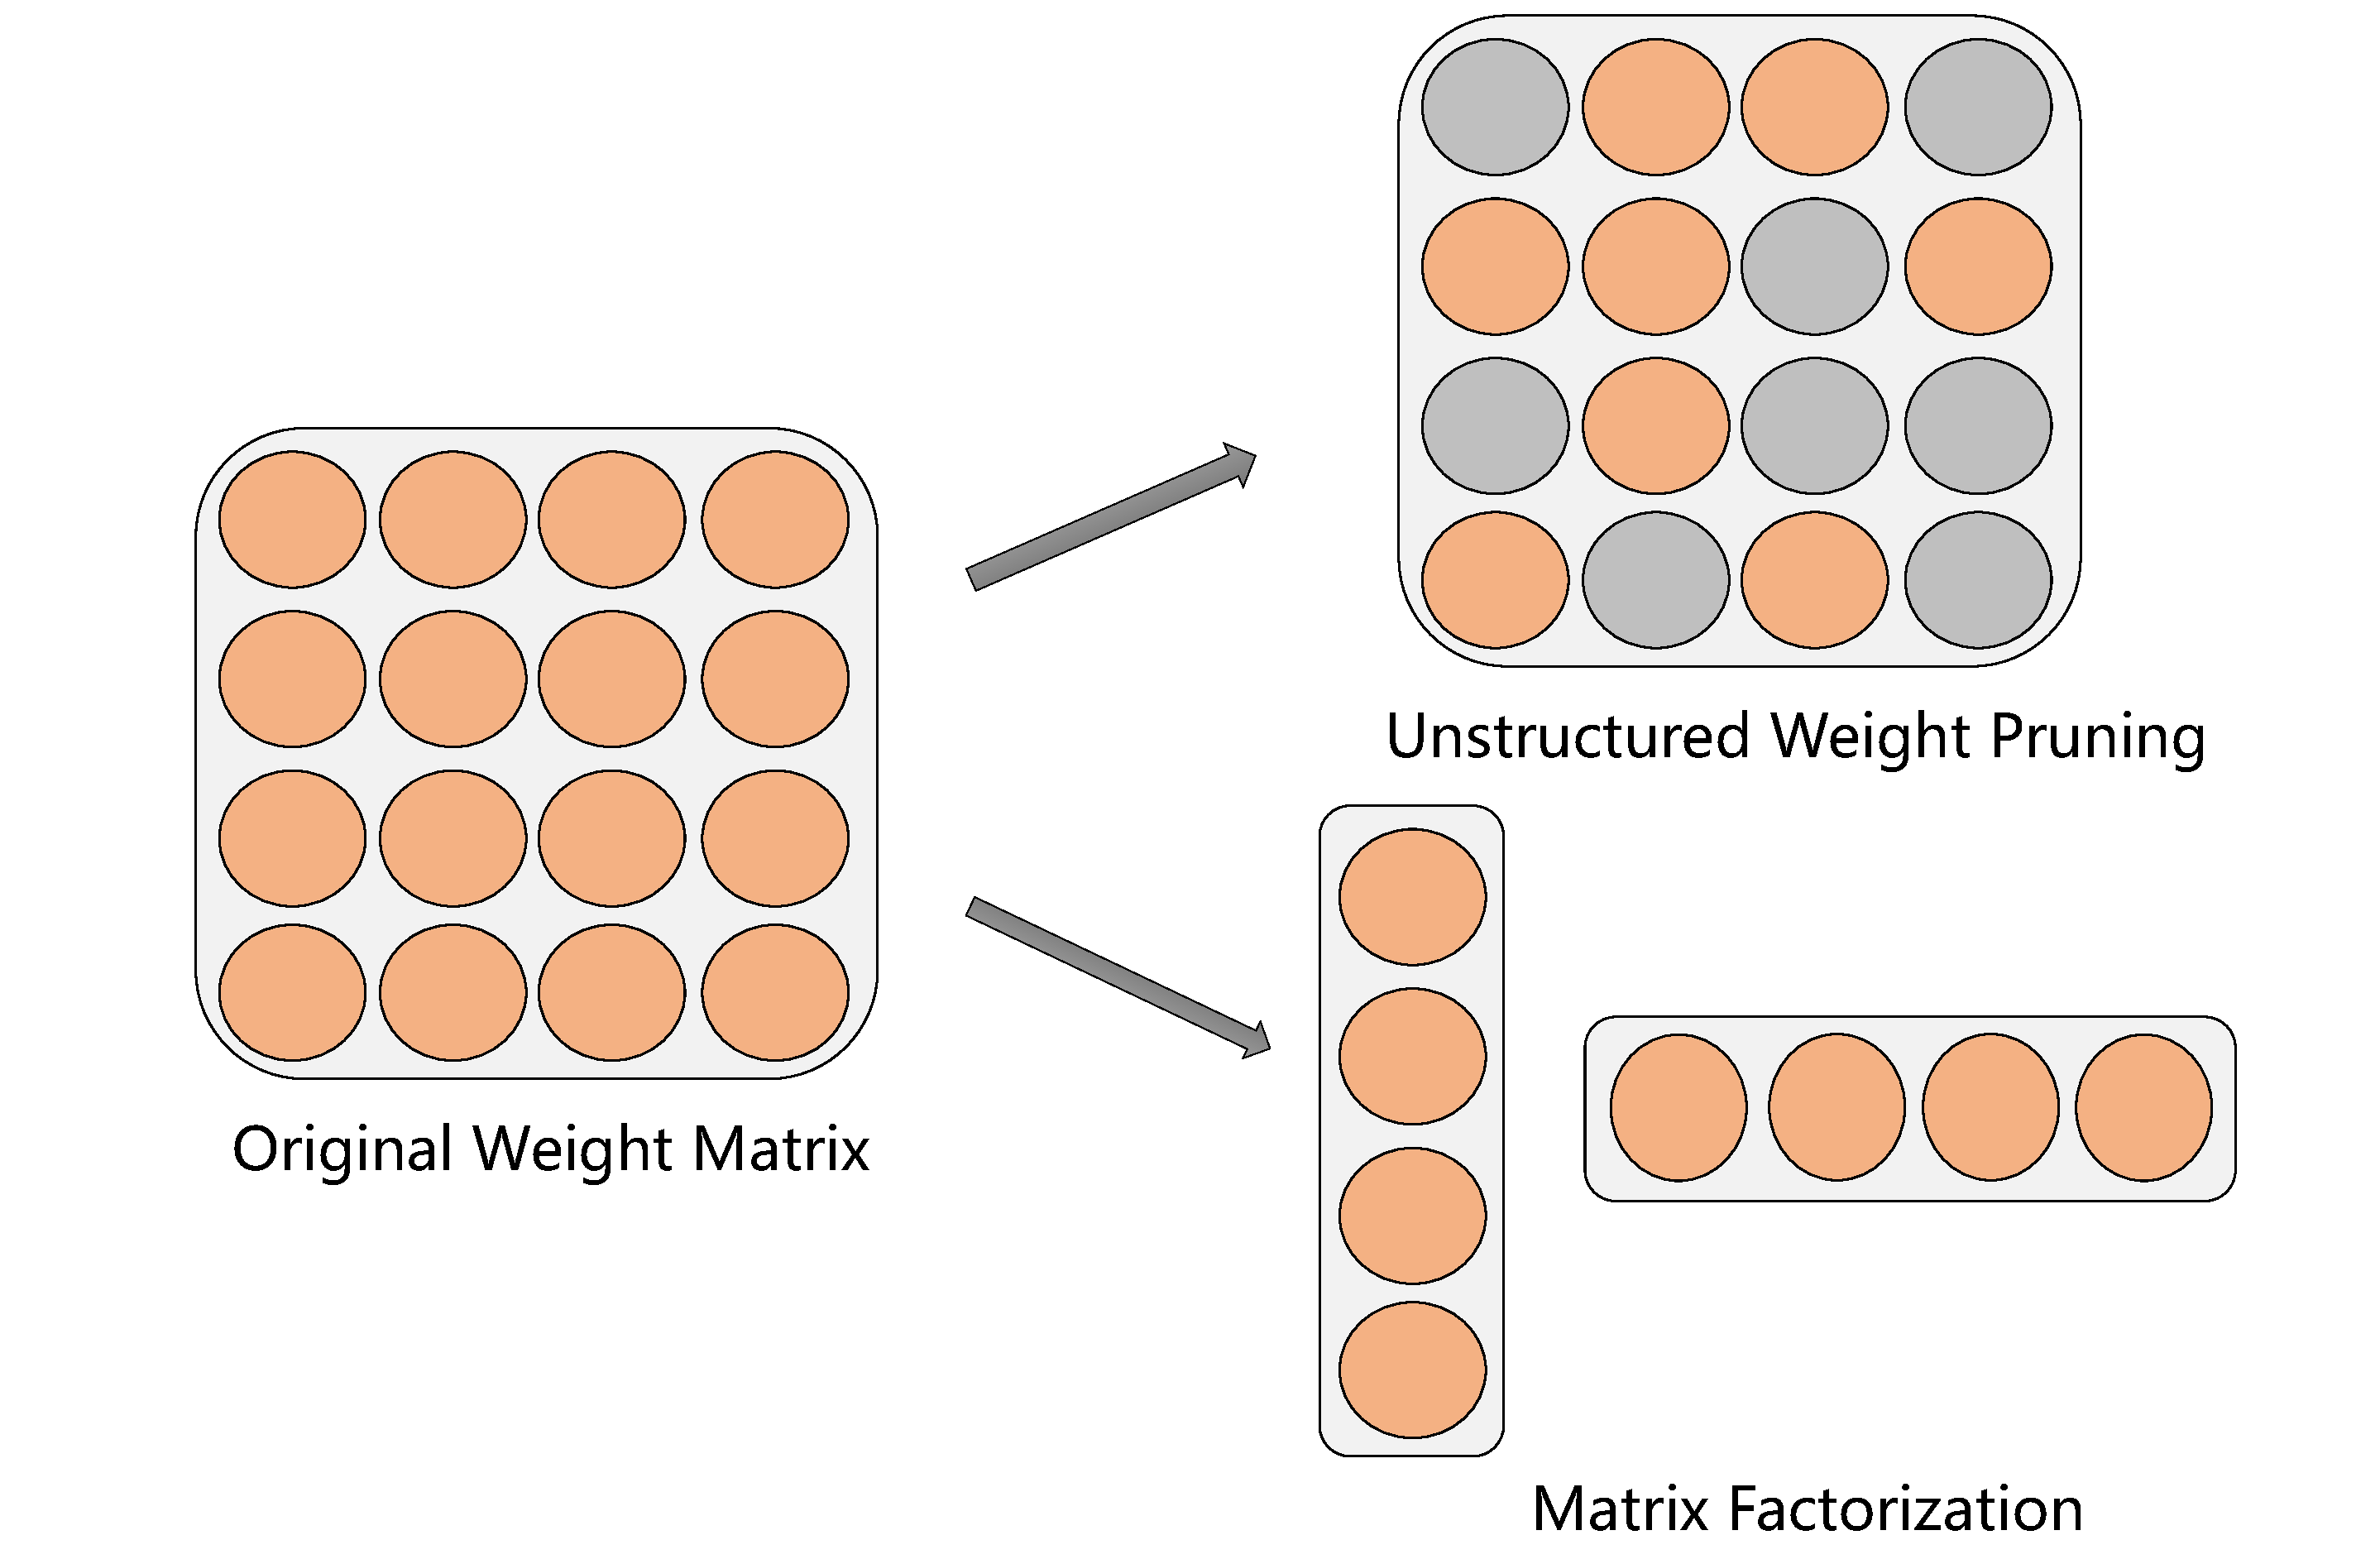
\includegraphics{./figures/intro_final.pdf}}
	\caption{Illustration of matrix factorization and unstructured pruning  on a single weight matrix.}
	\label{fig:intro}
\end{figure}

\subsection{Matrix Factorization~(MF)}
\label{sec:lr}
Given the weight matrix $\bm{W}\in \mathbb{R}^{n\times m}$, matrix factorization~\cite{svd} decomposes it into sub-matrices with reduced total number of parameters to achieve model compression.  
It first uses singular value decomposition~(SVD) to obtain an equivalent 
form of $\bm{W}$ as the product of three matrices:
\begin{align}
	\bm{W}=\bm{U}\bm{\Sigma}\bm{V}^\mathrm{T}
\end{align}
where $\bm{U}\in \mathbb{R}^{n\times r}$, $\bm{\Sigma}\in  \mathbb{R}^{r\times r}$, $\bm{V}\in \mathbb{R}^{r\times m}$, and $r$ is the rank of matrix $\bm{W}$. $\bm{\Sigma}$ is a diagonal matrix of non-zero singular values $\{\sigma_1, \sigma_2,...,\sigma_r\}$ in descending order. Then, low-rank approximation with targeted rank $k$ is obtained by keeping the top-$k$ singular values in $\bm{\Sigma}$ as well as their corresponding column vectors in $\bm{U}$ and $\bm{V}$:
\begin{align}
	\bm{W}&\approx \bm{U}_{[:, :k]}\bm{\Sigma}_{[:k,:k]}\bm{V}_{[:, :k]}^{\mathrm{T}} =\bm{A}\bm{B}
	\label{eq:svd}
\end{align}
where $\bm{A}=\bm{U}_{[:,:k]}\bm{\Sigma}_{[:k,:k]}$ and $\bm{B}=\bm{V}_{[:,:k]}^{\mathrm{T}}$ are the two final sub-matrices of which the product is used to replace $\bm{W}$. After such factorization, the number of parameters is reduced from $nm$ to $k(n+m)$. Different compression rates can be achieved by varying the preserved rank $k$.



\subsection{Unstructured  Pruning~(UP)}
\label{sec:pruning}
%We first establish some shared notations for unstructured weight pruning. 
Let $\bm{W}\in \mathbb{R}^{n\times m}$ denote a generic weight matrix in a PLM. In order to determine which elements in $\bm{W}$ are pruned, an importance score matrix $\bm{S}\in \mathbb{R}^{n\times m}$ is correspondingly introduced. The smaller $S_{i,j}$ is, the larger the probability of $W_{i,j}$ will be pruned. Given the importance scores, a pruning strategy $f_{prune}(\cdot)$ computes a binary mask matrix $\bm{M}\in \{0,1\}^{n\times m}=f_{prune}(\bm{S})$, 
and the forward process for an input $x$ becomes $y=(\bm{W}\odot\bm{M})x$, 
where $\odot$ denotes element-wise multiplication.

\paragraph{Zero-order Pruning~(UP$_{\text{zero}}$)} Zero-order pruning refers to the family of algorithms that only use the value of the weight as the importance measure.
For example, magnitude-based weights pruning~\cite{mag,chen2020lottery} adopts the absolute value of weight as importance score, i.e., 
$\bm{S}_{i, j}=|\bm{W}_{i, j}|$. The typical choice of $f_{prune}(\cdot)$ is to keep $v\%$  of weights with the largest importance scores:
\begin{align}
	\bm{M}_{i,j}=
	\begin{cases} 
		1, & \text{if }\bm{S}_{i,j}~\text{is in the largest }v\%\\
		0,  & \text{otherwise}  
	\end{cases}
	\label{eq:zero}
\end{align}


\paragraph{First-order Pruning~(UP$_\text{first}$)} Unlike zero-order pruning where $\bm{S}$ is directly derived from $\bm{W}$, first-order methods treat 
$\bm{S}$ as learnable parameters and jointly train it with model weights 
during fine-tuning. For example, SMvP~\cite{movement} and CAP~\cite{cap}
randomly initialize $\bm{S}$ and update it during the whole pruning process. The pruning strategy $f_{prune}(\cdot)$ is the same as in zero-order pruning~(\eqnref{eq:zero}).



Since the gradient of the thresholding function is 0 everywhere, straight-through estimator~\cite{st} is used as an approximation. The importance score $\bm{S}_{i,j}$ of $\bm{W}_{i,j}$ up to training step $T$ can be expressed as: 
\begin{align}
\bm{S}_{i,j}=-\sum_{t\le T}(\frac{\partial \mathcal{L}}{\partial \bm{W}_{i,j}})^{(t)} \bm{W}_{i,j}^{(t)}
\end{align}
where $\mathcal{L}$ is the loss function. The formulation is also equivalent to the first-order Taylor approximation of the change in $\mathcal{L}$ if $\bm{W}_{i,j}$ is zeroed out.

\paragraph{Sparsity Scheduler}
The proportion of remaining weights is controlled by the sparsity scheduler, here  we adopt the commonly used  cubic sparsity schedule to progressively reach target sparsity, i.e., $v_t$ at time step $t$ is derived by:
\begin{align}
	%	v^{(t)}=
	\begin{cases} 
		v_i & t\in [0, t_i) \\
		v_f+(v_i-v_f)(\frac{T-t_{f}-t}{T-t_f-t_i})^3 & t\in[t_i, T-t_f) \\
		v_f  & \text{otherwise}  
	\end{cases}
\end{align}
\label{eq:prune}
where $v_i=1.0$, $v_f$ is the final percent of remained parameters, $t_i$ and $t_f$ are the warmup and cool-down steps. $T$ is the total training steps. Moreover, we discard $\bm{M}$ and directly set $\bm{W}_{i,j}$ to zero if $\bm{S}_{i,j}^{(t)}$ is not in the top-$v_t$ at time step $t$. 
%\paragraph{A Unified View} The differences in the implementation of 
%importance scores~(direct value inspection v.s. additional learnable 
%parameters) and pruning strategy~(top-$v$ selection v.s. tuned threshold) 
%make it hard to compare various pruning methods. To this end, 
%we establish a unified view of zero-order and first-order pruning, 
%denoted as \textbf{UWP$_\text{zero}$} and \textbf{UWP$_\text{first}$}, 
%with the only difference being the calculation of importance score $\bm{S}$.
%\KZ{This section is a little strange here because it seems to repeat
%what has been said in the previous subsections. You have already defined $S$
%but now you are singling out $S$ again. In particular, I can't appreciate why
%``it is hard to compare various pruning methods'', I don't really see
%the need for this unified view.}
%
%For UWP$_\text{zero}$, the calculation of $\bm{S}$ is the same as magnitude pruning, i.e., $\bm{S}_{i, j}^{(t)}=|\bm{W}_{i, j}^{(t)}|$, where $t$ is the time step. For UWP$_\text{first}$, we directly calculate its importance score $\bm{S}$ without introducing additional parameters, i.e.,  $\bm{S}_{i,j}^{(t)}=\bm{S}_{i,j}^{(t-1)}+|\frac{\partial \mathcal{L}}{\partial \bm{W}_{i,j}}^{(t)} \bm{W}_{i,j}^{(t)}|$. 

%\KZ{\eqref{eq:prune} seems 
%to be something new in this section but then it is part of the first-order 
%pruning, and nothing to do with zero-order pruning. So why is it in the 
%``unified view?''}

%\KZ{My feel is that this whole section of related work and background is a bit
%long-winded.}
 


\section{Preliminary Study}
\label{sec:pilot}
In this section, we conduct a preliminary study on unstructured pruning  and matrix factorization
based on BERT-base and try to find answers to the following two questions: (1) How does matrix factorization perform under high compression rates? (2) Do subnetworks produced by unstructured pruning contain \textit{low-rank} sparsity patterns while preserving the majority of task accuracy?
%\KZ{What kind of insight? You stop short of providing the motivation
%of the following experiments. Are you trying to see if these two methods alone
%work well to compress language model?}

\subsection{Experimental Setting}
\indent
\paragraph{Datasets}We use two tasks from GLUE benchmark~\cite{glue}, namely MRPC and RTE, as our evaluation testbeds. Both of them are formulated as classification problems.

\paragraph{Implementation Details} For matrix factorization, we follow the algorithm in \secref{sec:lr}. Specifically, we first fine-tune BERT-base on each downstream task following \citet{bert}. Then, we perform truncated SVD on weight matrices of each linear layer in the fine-tuned BERT and re-train the whole model to recover the lost accuracy. We select preserved rank $k$ from $\{390, 260, 130, 50\}$, which corresponds to $\{0.75, 0.50, 0.25, 0.10\}$ of BERT's parameters.

For unstructured  pruning, we evaluate both UP$_\text{zero}$ and UP$_\text{first}$. We set the value of $v_f$ from $\{0.75, 0.50, 0.25, 0.10\}$ to make a direct comparison to matrix factorization.

\subsection{Results and Analysis}
\label{sec:pilot_results}

%\begin{figure*}[t]
%	\centering
%	\scalebox{0.285}{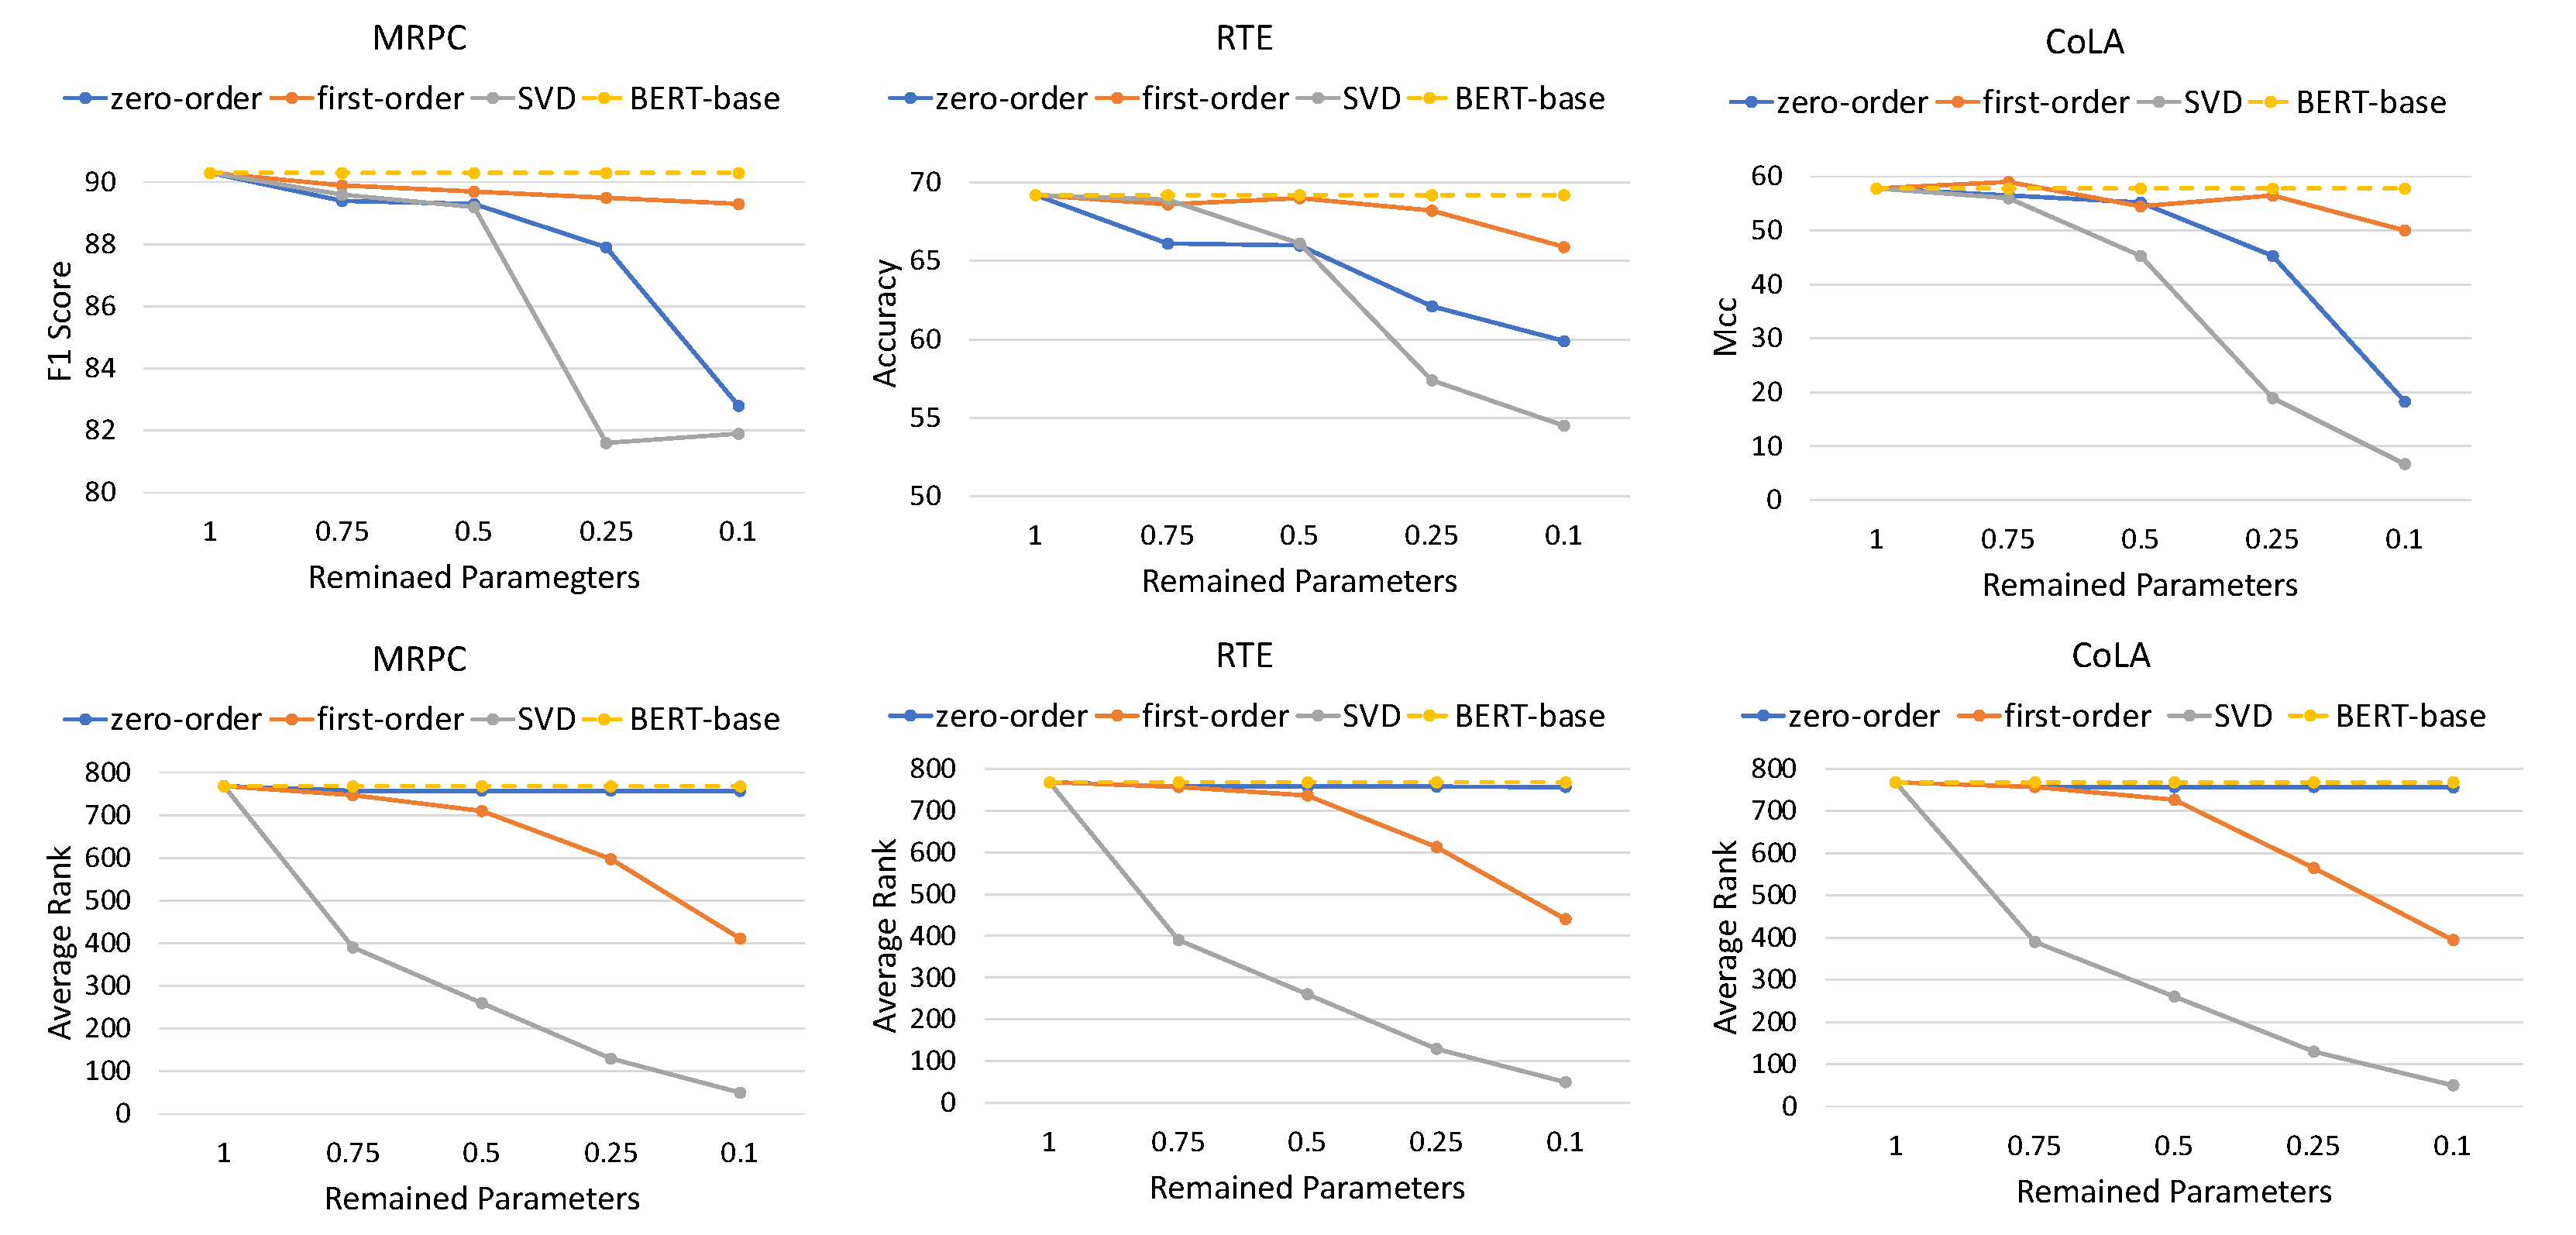
\includegraphics{./figures/pre_new.pdf}}
%	\caption{Task performance~(top half) and average matrix rank~(bottom half) v.s. percent of remained parameters. The dashed yellow line indicates the performance/rank upper bound by fine-tuning the full-scale BERT-base model.}
%	\label{fig:pre}
%\end{figure*}


\paragraph{Accuracy Preservation} 
The variation of task accuracy with respect to the remaining parameters is illustrated 
in the top half of \figref{fig:pre}. Under a small compression rate, i.e., 
$75\%$  parameters remaining, all examined methods can retain $\ge 97\%$ performance 
of BERT-base across all tasks. Under moderate compression rate, i.e., $50\%$ parameters remaining, UP$_\text{zero}$ and SVD start to show obvious declines. 
When more extreme compression rates are pursued, e.g., $25\%$-$10\%$ parameters 
remaining, SVD exhibits the most drastic performance drops compared to UP methods. 
On the contrary,  UP$_\text{first}$ still retains $\sim 97.6\%$ of BERT's performance.
UP$_\text{zero}$ lags behind UP$_\text{first}$ by a large margin under high sparsity. This indicates that magnitude alone cannot be used to quantify a weight's 
contribution because even a small weight can yield a huge influence on the model 
output due to the complicated compositional nature of neural networks. 
In contrast, the importance criterion of UP$_\text{first}$ directly reflects the 
sensitivity of the model's training loss w.r.t. each weight and is therefore more 
accurate.

\begin{figure}[t]
	\centering
	\scalebox{0.175}{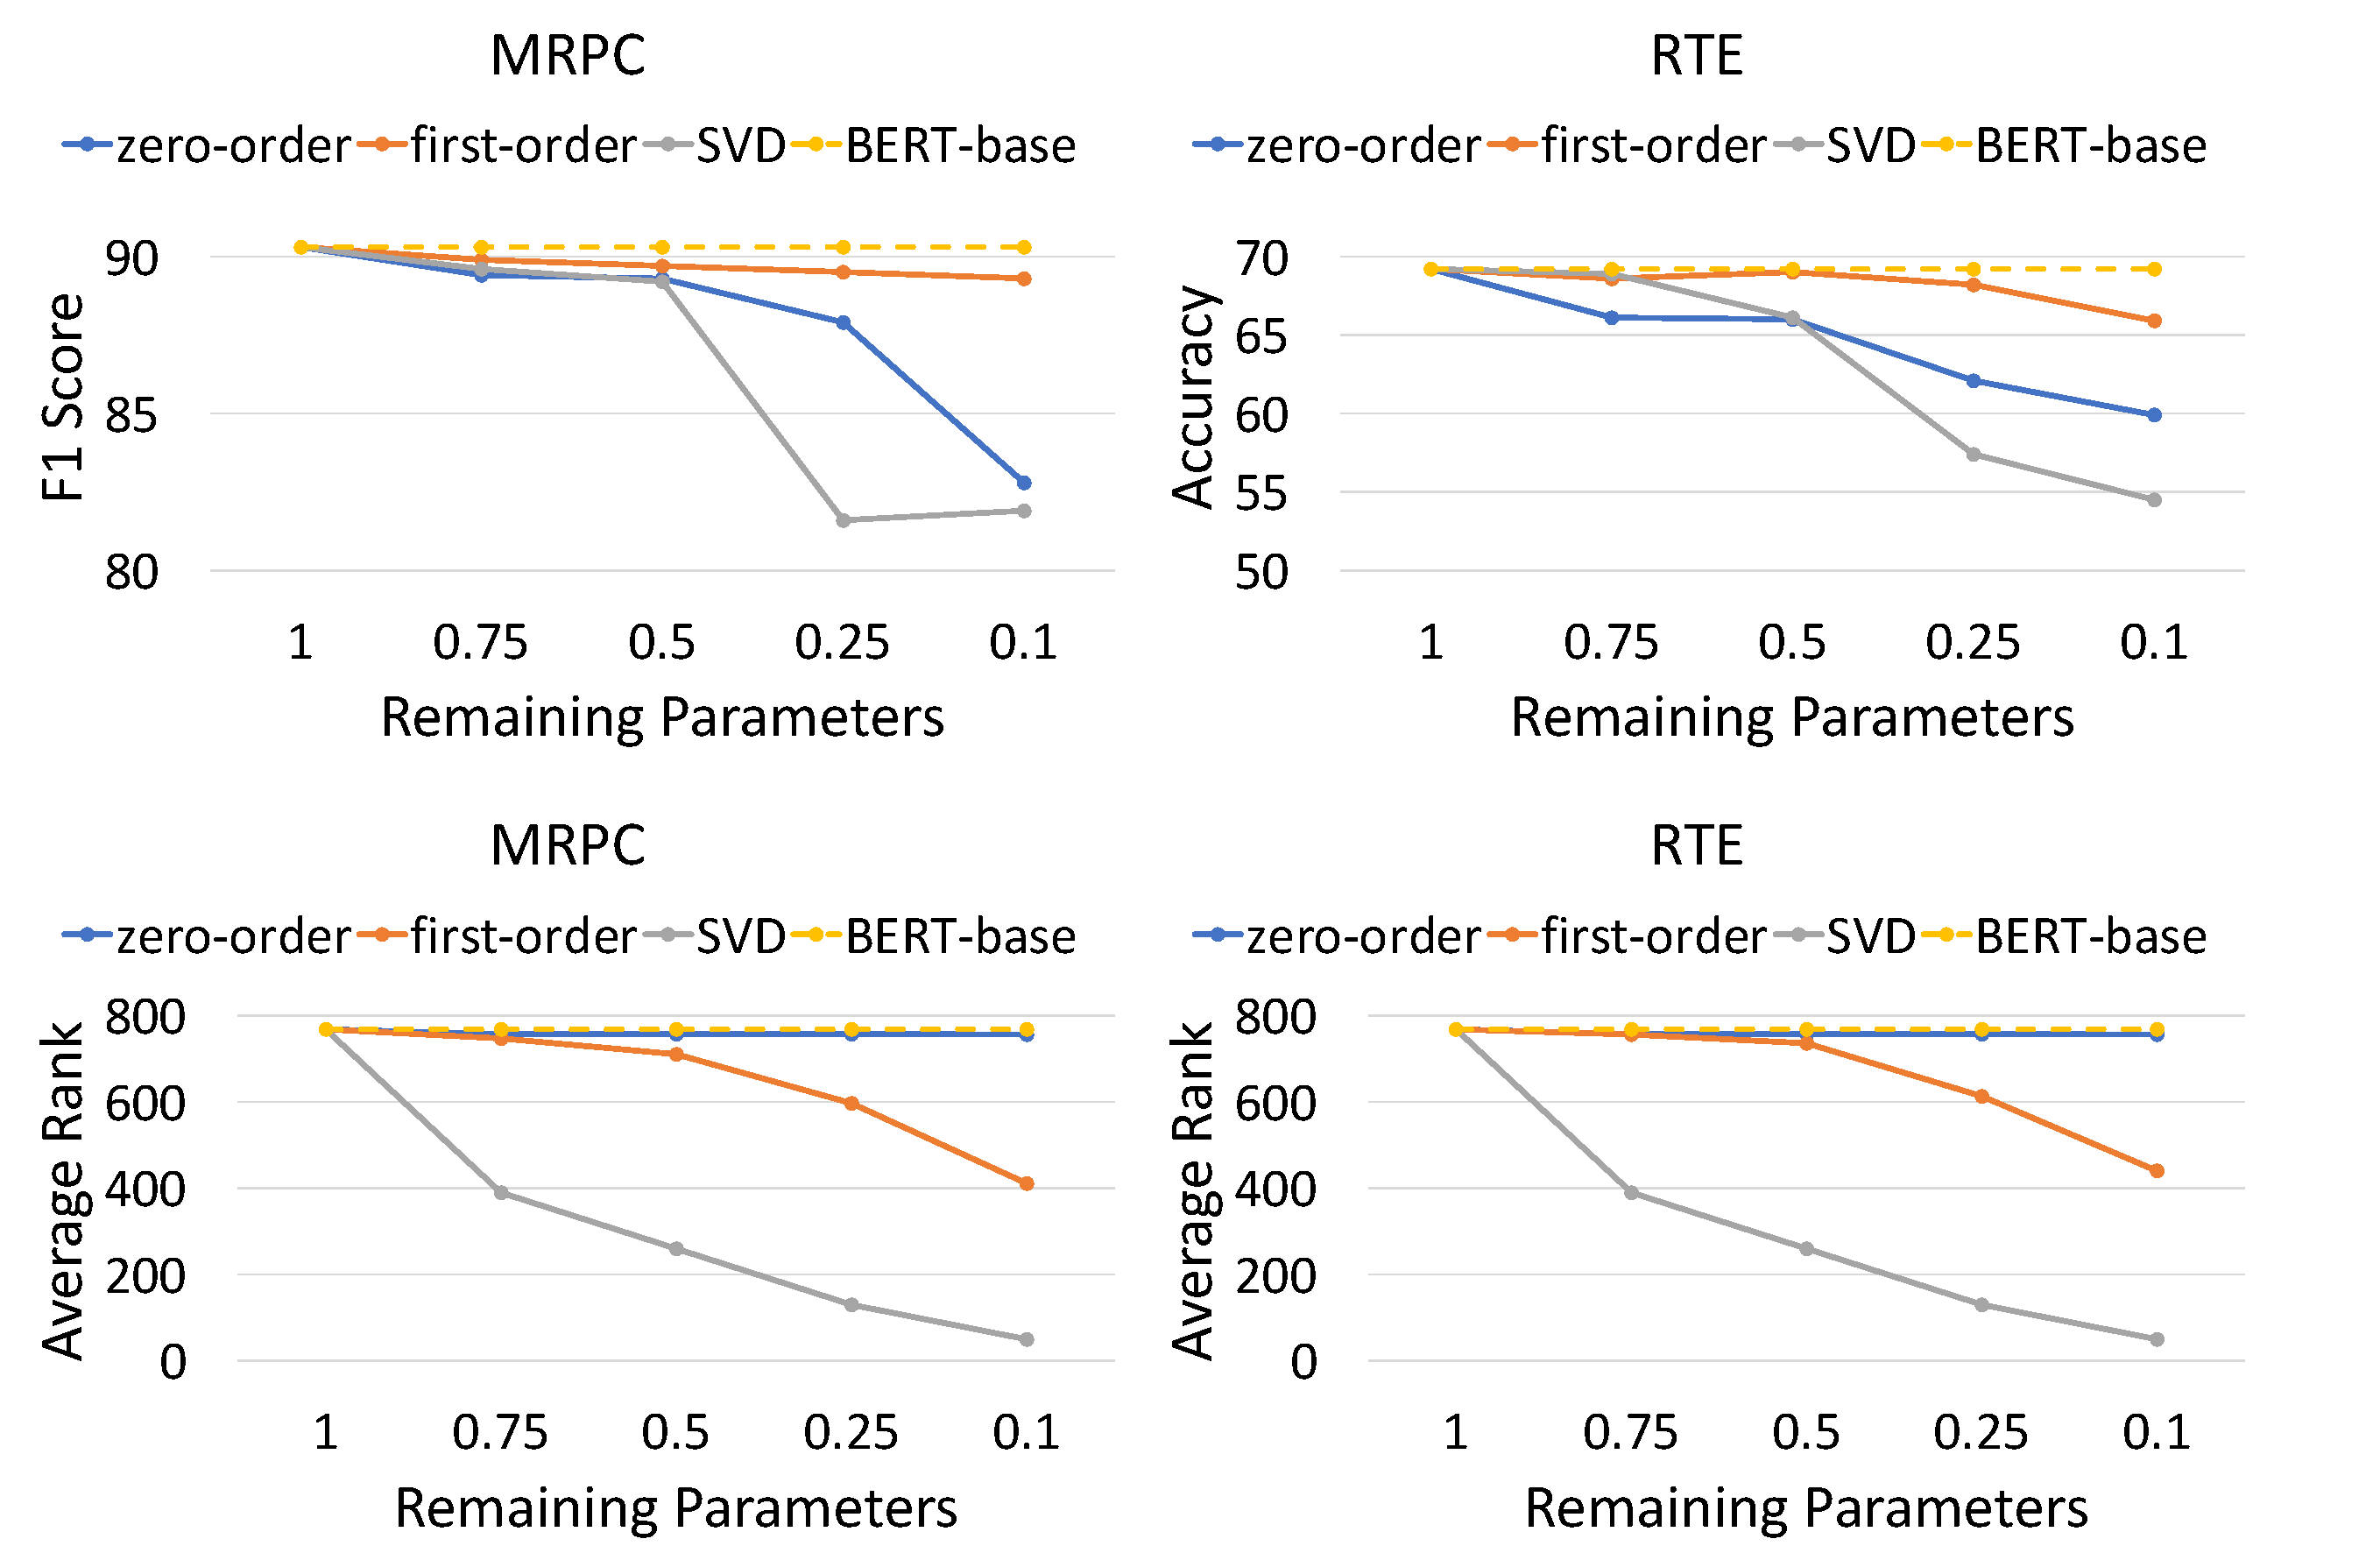
\includegraphics{./figures/pre_col.pdf}}
	\caption{Task accuracy~(top half) and average matrix rank~(bottom half) 
v.s. percentage of original parameters retained. 
The dashed line indicates the performance/rank upper bound by fine-tuning the full-scale BERT-base model.}
	\label{fig:pre}
\end{figure}

\begin{figure}[t]
	\centering
%	\scalebox{0.50}{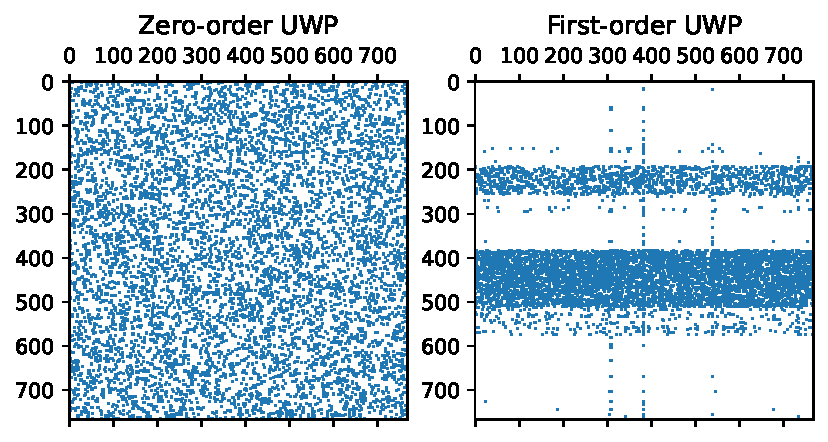
\includegraphics{./figures/sparsity_pattern.pdf}}
		\scalebox{0.50}{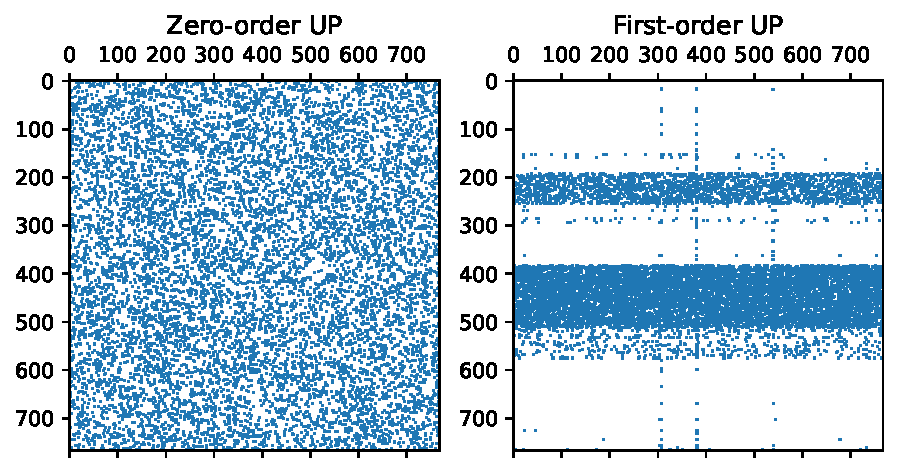
\includegraphics{./figures/zero_first_UP.pdf}}
	\caption{Sparsity patterns of the same 768x768 weight matrix  pruned by UP$_\text{zero}$~(left) and UP$_\text{first}$~(right) on MRPC with $10\%$ of
the parameters remaining.}
	\label{fig:pattern}
\end{figure}

\paragraph{Rank} 
Considering the inferior accuracy of SVD, we hypothesize that the weight matrices of fine-tuned BERT are high-rank, 
hence leading to a large approximation error when $k$ is small. The bottom half of \figref{fig:pre} inspects the average rank of weight matrices. We can see that the weight matrices in fine-tuned BERT-base are nearly full-rank, which explains the inefficacy of SVD when $k$ is small. We also plot the rank-parameter curve of UP methods. For UP$_\text{zero}$, it produces sparse matrices that are 
as high-rank as densely fine-tuned BERT even when $90\%$ weights are set to zero. In contrast, UP$_\text{first}$  produces sparse patterns whose rank monotonically decreases as more weights are pruned. To gain more insights into this phenomenon, we visualize the weight matrix pruned by UP$_\text{zero}$ and UP$_\text{first}$ in \figref{fig:pattern}. Though both are designed without structural bias,  unlike UP$_\text{zero}$, UP$_\text{first}$ learns to remove entire rows from the weight matrix and 
the resulting matrix enjoys a low-rank characteristic.



\begin{figure}[th]
	\centering
	\scalebox{0.142}{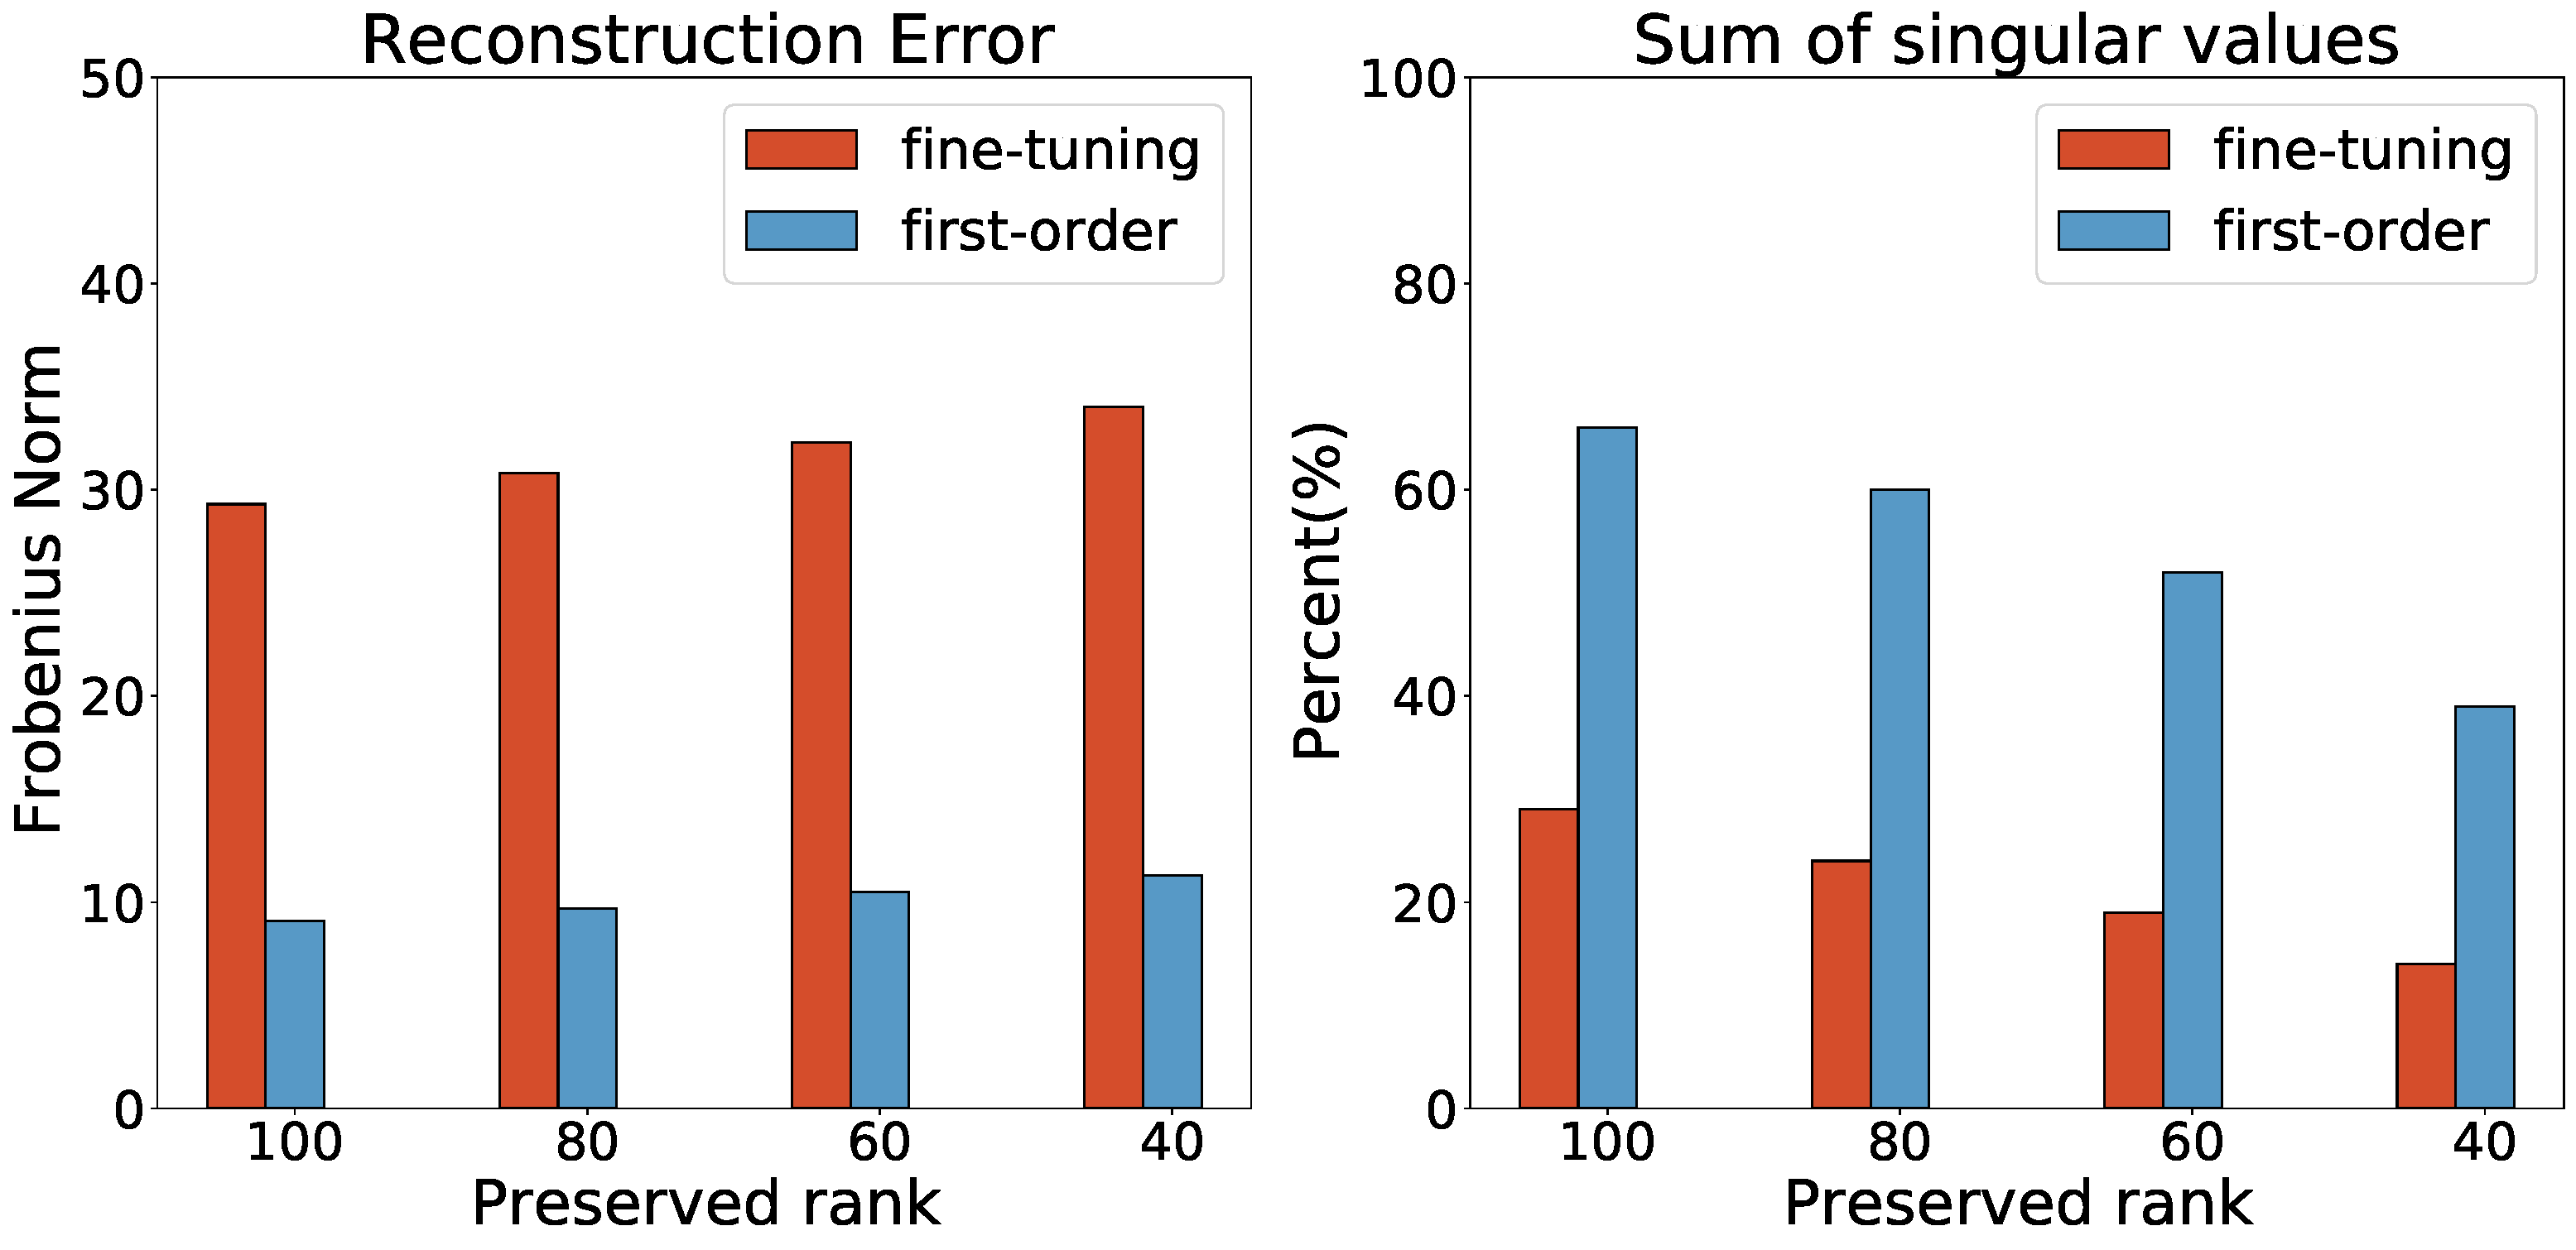
\includegraphics{./figures/norm_vis.pdf}}
	\caption{Quantitatively measuring approximation quality via reconstruction error~(left) and cumulative sum of singular values~(right) on MRPC.}
	\label{fig:norm}
\end{figure}

\paragraph{The Idea}
%\KZ{The key insight is: factorize a high-rank matrix into low rank sub-matrices
%loses a lot of info, but factorize a low-rank matrix into low rank sub-matrices
%doesn't lose as much info. Our design is based on this insight. I think as long
%as you make this insight clear, that's good enough. Some of this section
%is a bit verbose.} 
%Given the fact that factorizing from a low-rank matrix into sub-matrices loses less information than factorizing from a high-rank matrix
%Given the competitive task performance and low-rank structure of UWP$_\text{first}$, 
%it appears plausible to perform low-rank matrix factorization on 
%low-rank sparse models for model compression. 
The key insight is: factorizing a high-rank matrix into low rank sub-matrices
loses significant quantity of useful information, but factorizing a low-rank matrix into low rank sub-matrices
doesn't lose as much information. Our design is based on this insight. 
As a sanity check of its feasibility, we quantitatively measure the 
quality of low-rank approximation with various preserved ranks $k$. 
\figref{fig:norm} shows that given a specific $k$, 
the sum of top-$k$ singular values of matrices produced by UP$_\text{first}$ takes a much larger portion of total values than fine-tuning, suggesting that we can reserve more information of low-rank sparse matrix given the same $k$. The reconstruction error~(measured by Frobenius norm) of UP$_\text{first}$ is also significantly lower, implying a higher approximation quality. We thus expect that low-rank matrix factorization on low-rank sparse models to effectively combine: 
(1) the good performance of first-order UP; 
(2) direct memory and computation reduction by MF.

\section{LPAF: Low-rank Prune-And-Factorize}
\label{sec:approach}
Here we formally propose the LPAF~(\textbf{L}ow-rank \textbf{P}rune-\textbf{A}nd-\textbf{F}actorize) framework 
for language model compression. In addition, 
we propose two optimizations in the 
initialization and training of the compression process.

\subsection{The Overall Workflow}
\label{sec:ptf}
Given a pre-trained language model $T$ and a downstream task with training set $D=\{(x_i, y_i), i=1,2,...M\}$, LPAF consists of three steps to realize model compression: 
\begin{itemize}
	\item Step-1: obtaining the low-rank sparse model $T_{\text{sparse}}=\text{UP}_\text{first}(T,D, v)$. $v$ is the percent of remained parameters after pruning.
	\item Step-2:  performing matrix factorization on each weight matrix~(excluding the embedding layer) in $T_{\text{sparse}}$ and  obtain its low-rank factorized form $T_{\text{factorized}}$. 
	\item Step-3:  re-training $T_{\text{factorized}}$ on $D$ using task-specific loss function until convergence. 

\end{itemize}

Next, we present two novel optimizations, namely \textit{sparsity-aware SVD} and \textit{mixed-rank fine-tuning}, that improve the matrix factorization and fine-tuning process in step 2 and step 3 respectively.

\subsection{Optimization 1: Sparsity-aware SVD}
\label{sec:sasvd}
SVD has been shown~\cite{bestsvd} to provide the optimal rank-$k$ approximation to $\bm{W}$ with respect to the Frobenius norm:
\begin{align}
	\nonumber
	\min_{\bm{A},\bm{B}} ||\bm{W}-&\bm{A}\bm{B}||_{F}=\min_{\bm{A},\bm{B}} \sum_{i,j}(\bm{W}_{i,j}-(\bm{AB})_{i,j})^2 \\
	& \text{s.t.}~~~~\text{rank}(\bm{AB})=k
\end{align}
It is a generic factorization method in that it is applicable to any matrix $\bm{W}$ by penalizing the reconstruction error of each individual weight equally. 

In our case, $\bm{W}$ is a sparse matrix from $T_{\text{sparse}}$ in which the majority of weights are set to zero by the pruning algorithm $P$. These zero weights are deemed to have less impact on the task performance compared to the retained~(unpruned) weights. However, the vanilla SVD treats each weight equally without considering the inherent sparseness of $W$, thus may be sub-optimal for preserving useful information in $W$ about the end task.
To address this issue, we propose sparsity-aware SVD which considers different priorities of parameters and weighs the individual reconstruction error based on its importance score $\bm{S}_{i,j}$:
\begin{align}
	\min_{\bm{A},\bm{B}} \sum_{i,j}&\bm{S}_{i,j}(\bm{W}_{i,j}-(\bm{AB})_{i,j})^2~~~\\\
	 & \text{s.t.}~~\text{rank}(\bm{AB})=k
	\label{eq:sasvd}
\end{align}
In this way, parameters that are more important can be better reconstructed, hence retaining more task performance from $T_{\text{sparse}}$ at initialization. Nevertheless, \eqnref{eq:sasvd} does not have a closed form solution~\cite{weightedsvd,hsu2021language} when each $\bm{W}_{i,j}$ has its own weight. We therefore resort to a simplification by letting the same row of $\bm{W}$ share the same importance. The importance for row $i$ is given by $\hat{\bm{S}}_{i}=\frac{\sum_{j}\bm{S}_{i,j}}{\sum_{n}\hat{\bm{S}}_{n}}$. Let $\hat{\bm{I}}=diag(\hat{\bm{S}}_1,\hat{\bm{S}}_2,...,\hat{\bm{S}}_{n})$ denote a diagonal matrix,  \eqnref{eq:sasvd} is now converted to:
\begin{align}
	&\min_{\bm{A},\bm{B}}||\hat{\bm{I}}\bm{W}-\hat{\bm{I}}\bm{A}\bm{B}||_F~~~~
	\\
	& \text{s.t.}~~\text{rank}(\bm{AB})=k
\end{align}
This essentially amounts to applying rank-$k$ SVD upon $\hat{\bm{I}}\bm{W}$, i.e., $\hat{\bm{I}}\bm{W}=\hat{\bm{U}}\hat{\bm{\Sigma}}\hat{\bm{V}}^\mathrm{T}$. Then the solution of $\bm{A}$ and $\bm{B}$ can be analytically obtained by:
\begin{align}
	\bm{A} &= \hat{\bm{I}}^{-1}\hat{\bm{U}}_{[:,:k]}\hat{\bm{\Sigma}}_{[:k,:k]},\bm{B}=\hat{\bm{V}}_{[:,:k]}^{\mathrm{T}}
\end{align}


\subsection{Optimization 2: Mixed-rank Fine-tuning}
Recall that the last step of LPAF is to fine-tune $T_{\text{factorized}}$ on the training set $D$. This process has been proven essential to regain the performance lost during factorization~\cite{svd}. However, during the experiments, we observe the performance of fine-tuned $T_{\text{factorized}}$ still slightly lags behind $T_{\text{sparse}}$ given a similar parameter budget. 
%\KZ{Isn't it normal for $T_{factorize}$ to lag behind $T_{sparse}$? Is there any evidence (experimental results) to show
%this ``lagging''?  Even in Fig. 3, in most cases, $T_{sparse}$ is still better Ours. 
%So I don't see enough motivation for this Mixed-rank fine-tuning.} 
We posit that, due to the reduced capacity~(less trainable parameters) and model-level approximation error incurred by low-rank factorization, joint fine-tuning of low-rank matrices may converge to sub-optimal solutions with lower generalization ability. To mitigate this problem, we propose mixed-rank fine-tuning, a regularized scheme for training low-rank matrices.

Let $\{(\bm{A}\bm{B})_i, i=1,2...,N\}$ denotes all low-rank matrices in $T_{\text{factorized}}$. During training, for each $(\bm{A}\bm{B})_i$, we sample a binary Bernoulli random variable $z_i\sim \text{Bernoulli}(p)$, where $p$ is a global hyper-parameter. Then, the local computation process involving $(\bm{A}\bm{B})_i$ is modified to:
\begin{align}
	\bm{x}_{out} = (1-z_i)*(\bm{A}\bm{B})_i \bm{x}_{in} + z_i * \bm{W}_i\bm{x}_{in} 
\end{align}
where $\bm{W}_i$ is the sparse matrix in $T_{\text{sparse}}$ from which $\bm{A}_i$ and $\bm{B}_i$ are derived. In this way, the low-rank matrices can further 
benefit from gradient-level regularization from  $T_{\text{sparse}}$, 
thus reducing the generalization gap. The hyper-parameter $p$ is controlled by a scheduler. We implement it such that $p$ is linearly decayed from an initial value $p_{\text{init}}$ to zero by a constant step size $d$:
\begin{align}
	p = \text{max}(0, p_{\text{init}}-d*t)
\end{align}
As $p$ decreases, $\bm{W}_i$ is gradually substituted by low-rank sub-matrices $(\bm{AB})_i$. When $p$ reaches zero, the training enters the phase of standard fine-tuning. To further mitigate the training instability brought by sampling, we let each input go through the forward pass twice with different $\bm{z}^1=\{z_i^1\}_{i=1}^{N}$ and $\bm{z}^2=\{z_i^2\}_{i=1}^{N}$, and impose a consistency objective on the two outputs to promote stability:

\begin{align}
	\mathcal{L}_{c}=\mathcal{D}(y_{\bm{z}^1}, y_{\bm{z}^2})
\end{align}
where $\mathcal{D}$ can be the KL divergence for classification tasks and the MSE loss for regression tasks.

% After $p$ reaches zero, the model still benefits from the regularization effect brought by different dropout masks~\cite{rdrop}.
